% =====================================================================
%  FedCoP: Federated Co-occurrence-aware Prototypes for
%          Multi-Label Medical Image Classification
%
%  Self-contained LaTeX source. Compile with pdflatex (run twice for refs).
%  Figures and experimental numbers are left as placeholders (marked
%  \TODO) to be filled from run logs.
% =====================================================================
\documentclass[11pt,a4paper]{article}

\usepackage[utf8]{inputenc}
\usepackage[T1]{fontenc}
\usepackage[margin=1in]{geometry}
\usepackage{amsmath,amssymb,amsthm}
\usepackage{mathtools}
\usepackage{graphicx}
\usepackage{booktabs}
\usepackage{multirow}
\usepackage{array}
\usepackage{xcolor}
\usepackage{enumitem}
\usepackage{caption}
\usepackage[numbers,sort&compress]{natbib}
\usepackage{hyperref}
\hypersetup{colorlinks=true,linkcolor=blue!60!black,citecolor=blue!50!black,urlcolor=blue!60!black}

% ---- theorem environments ----
\newtheorem{proposition}{Proposition}
\newtheorem{remark}{Remark}
\theoremstyle{definition}
\newtheorem{definition}{Definition}

% ---- lightweight TODO placeholder ----
\newcommand{\TODO}[1]{\textcolor{red!70!black}{[\textbf{TODO:} #1]}}

% ---- shortcuts ----
\newcommand{\Rhat}{\widehat{R}}
\newcommand{\Sigmay}{\Sigma_{y}}
\newcommand{\bc}{\boldsymbol{\mu}_c}
\newcommand{\sigc}{\boldsymbol{\sigma}_c^{2}}
\DeclareMathOperator*{\argmax}{arg\,max}

\title{FedCoP: Federated Co-occurrence-aware Prototypes for \\
       Multi-Label Medical Image Classification}
\author{
  Anonymous Authors\\
  \textit{[Affiliation]}\\
  \texttt{[email]}
}
\date{}

\begin{document}
\maketitle

% =====================================================================
\begin{abstract}
Federated learning lets hospitals train a shared model without exchanging patient data, and prototype-based federated learning sharpens this by sharing only class prototypes, which lowers communication cost and reduces the exposure of raw gradients. Yet every method in this line models each of the $C$ pathologies with an independent prototype and decodes labels with independent per-class sigmoids, which is equivalent to assuming the labels are conditionally independent given the features. That assumption is wrong for multi-label medical imaging, where diseases co-occur as a matter of physiology: pleural effusion accompanies atelectasis because fluid compresses lung tissue, and consolidation tracks infiltration in pneumonia. The assumption fails in a second, structural way under the realistic federated setting: when each hospital sees only a subset of the $C$ classes, no single client can observe the global co-occurrence structure at all, since the entries for any pair it never jointly sees are exactly zero rather than merely noisy. We argue that co-occurrence is therefore an intrinsically federated quantity, invisible to any participant and recoverable only by aggregation, and we make it a first-class object of the federation.

We propose \textbf{FedCoP} (Federated Co-occurrence-aware Prototypes). FedCoP augments distributional prototypes with a federatedly estimated co-occurrence correlation matrix $\Rhat$, and uses $\Rhat$ on both sides of the pipeline. On the training side, a structure loss $L_{co}$ aligns the inter-class prototype geometry (the cosine Gram matrix) to $\Rhat$, replacing the heuristic contrastive and adversarial regularizers of prior work with a single target driven by label statistics. On the inference side, a correlation-aware mean-field decoder propagates evidence across co-occurring classes, which is provably no worse than independent sigmoids and strictly better when $\Rhat$ tracks the residual label correlation. $\Rhat$ is estimated from privacy-safe label sufficient statistics $(\mathbf{m}_k,\mathbf{M}_k,n_k)$ aggregated by count-weighted, de-biased fusion. We prove two results: a decoder-regret bound showing the independent decoder is Bayes-optimal only under conditional independence, with regret $\Omega(\|\Sigmay-I\|_F^{2})$ that the mean-field decoder reduces to a variational gap; and a federated-estimation theorem giving unbiasedness under participation reweighting, matrix-Bernstein concentration at rate \allowbreak$\tilde O(\sqrt{\log C/(K n_{\min})})$, and single-client non-recoverability of the structure under non-IID class partitioning. We evaluate on two multi-label datasets of different modalities, NIH ChestX-ray14 (thoracic, radiography) and MuReD (retinal, fundus), under non-IID federated splits, and isolate the contributions of the federated structure, the training-side loss, the inference-side decoder, and six supplementary design choices through comprehensive ablations.
\end{abstract}

% =====================================================================
\section{Introduction}
\label{sec:intro}

Chest radiography is the most frequently performed imaging exam in medicine, and reading a film is naturally a multi-label problem: a single image often carries several findings at once. This is not an artifact of how the data is labeled but a reflection of physiology. Pleural effusion and atelectasis co-occur because fluid compresses lung tissue; consolidation and infiltration accompany pneumonia. A model that reads a chest film as fourteen independent yes-or-no questions is, clinically, reading it wrong. When such models are trained across hospitals under privacy constraints, the federated setting that medicine requires, the methods we have still treat the fourteen pathologies as independent. This paper addresses that gap and explains why the remedy must itself be federated.

\subsection{Prototype-based FL and its independence assumption}

Federated learning trains a shared model across hospitals without exchanging data \citep{mcmahan2017fedavg}. \textbf{FedProto} \citep{tan2022fedproto} replaced weight sharing with prototype sharing: each client uploads a per-class mean feature vector and the server averages them, while clients regularize their local features toward the global prototypes. This is communication-efficient, architecture-agnostic, and friendlier to privacy than sharing raw weights, which can in principle leak training data. For these reasons prototype sharing has become the dominant paradigm for privacy-sensitive federated learning, and follow-up work has strengthened the prototype \emph{representation} (Gaussian mixture heads \citep{zhang2024fedgmkd}, distributional heads) and the \emph{aggregation} (quality-weighted fusion \citep{zhang2024fedgmkd}, Bayesian fusion \citep{chen2021fedbe}).

Every method in this line, however, keeps two independence assumptions that are especially harmful in multi-label medical imaging:
\begin{enumerate}[leftmargin=*,itemsep=2pt]
  \item \emph{Storage and alignment independence.} The $C$ class prototypes are stored as a set $\{\mathbf{p}_c\}_{c=1}^{C}$ and the alignment loss treats each class in isolation. A sample carrying the co-occurring set \{Effusion, Infiltration\} produces two unrelated prototype-alignment gradients.
  \item \emph{Decoding independence.} Inference computes $p(y_c{=}1\mid \mathbf{x})=\sigma(-d_c(\mathbf{x})/T)$ independently per class.
\end{enumerate}
These are two faces of one assumption: the $C$ labels are conditionally independent given the features. The first face says prototype geometry need not reflect inter-class relations; the second says decoding need not propagate information across classes. In a domain where labels are strongly correlated and comorbidity is the norm, both faces are wrong, and the decoding face is provably suboptimal. We show in Section~\ref{sec:theory} that the independent sigmoid decoder is Bayes-optimal only under conditional independence and pays a regret that grows with the residual label correlation. In effect the field has built increasingly elaborate prototypes on top of a decoder that discards the very structure that makes multi-label medical imaging multi-label.

\subsection{The federated co-occurrence opportunity}

The obvious remedy, modeling label correlation, runs into an immediate obstacle in the federated setting, and that obstacle motivates the paper. The co-occurrence structure is non-local. Under the realistic non-IID class partitioning of federated medical data, each hospital sees only a subset of the $C$ pathologies ($\text{ways}<C$); a specialist center for effusion does not also see enough hernia cases to know how the two relate. Concretely, a client's co-occurrence count matrix $\mathbf{M}_k$ has zero rows and columns for every class it never sees, so the entries for any pair it does not jointly observe are exactly zero, not merely small. No amount of local data distinguishes ``these never co-occur'' from ``I never see these.''

This is a structural fact that dictates the solution rather than a mere inconvenience. The global $C\times C$ co-occurrence structure is recoverable only by federated aggregation of per-client sufficient statistics, across clients whose class supports jointly cover all $C$ classes. Co-occurrence is therefore a structurally federated quantity, invisible to any participant and visible only to the federation as a whole, rather than a multi-label technique that happens to run inside a federated system. The same necessity was observed by FedALC \citep{an2024fedalc} in the single-positive-label setting; our contribution lies not in the observation itself but in what follows from it: a general sufficient-statistic estimator with de-biasing and concentration guarantees (Proposition~\ref{prop:estimation}), and the use of the estimate on both prototype geometry and decoding.

\paragraph{Heterogeneity along four axes.}
The class-support gap is not the only axis on which federated medical data is non-IID; it is merely the one most directly responsible for co-occurrence. Three others accompany it, and each makes a different global quantity invisible to any single client. \emph{Marginal prevalence} varies: an effusion specialist sees effusion far more often than the global base rate, so its local $p_c$ is a biased view of $\pi_c$. \emph{Co-occurrence structure} itself varies: even for two classes a client does see, the local $\phi$ coefficient reflects that client's case mix, not the population. \emph{Participation} is unequal: clients contribute different counts $n_k$ at different rates, so naive averaging is biased toward over-participating clients. The common shape is the same: a quantity that is global by definition is observed only through biased local fragments and is recovered only by aggregation that corrects for the bias. FedCoP federates $\boldsymbol\pi$ and $\Rhat$ together from the same sufficient statistics; for settings with severely imbalanced participation, importance reweighting by $1/\pi_k$ can restore unbiasedness (Proposition~\ref{prop:estimation}a).

\subsection{Contributions}

\begin{enumerate}[leftmargin=*,itemsep=2pt]
  \item \textbf{Federated co-occurrence structure.} A privacy-safe, count-weighted estimator of the global pathology co-occurrence correlation $\Rhat$ from label sufficient statistics $(\mathbf{m}_k,\mathbf{M}_k,n_k)$, with $\phi$-correlation de-biasing, shrinkage, and EMA smoothing. The estimator is unbiased under reweighted participation and concentrates at rate \allowbreak$\tilde O(\sqrt{\log C/(K n_{\min})})$.
  \item \textbf{Correlation-aware prototypes.} A training-side structure loss $L_{co}$ aligning the prototype cosine Gram to $\Rhat$, and an inference-side mean-field decoder using $\Rhat$, together replacing the heuristic contrastive and adversarial regularizers of prior prototype-FL with a single, label-statistics-driven mechanism that acts on both sides of the pipeline.
  \item \textbf{Theory.} A decoder-regret bound showing the mean-field decoder is never worse than independent sigmoids and strictly better when $\Rhat$ tracks the residual label correlation; and a federated-estimation theorem (unbiasedness, matrix-Bernstein concentration, single-client non-recoverability) that formalizes, for the general non-IID class-partition setting, why the structure must be federated.
  \item \textbf{Minimal method and stronger evaluation.} A deliberately minimal four-loss objective that omits per-class temperature, adversarial, contrastive, and calibration losses (analyzed as redundant or dead), a FedProx baseline, and full multi-label metrics (macro/micro AUROC, F1, Hamming loss, subset accuracy), with comprehensive ablations that separately isolate the federated structure, the training-side loss, the inference-side decoder, and six supplementary design choices (distributional vs.\ point prototypes, entropy regularization, logit fusion ratio, distance metric, and temperature scaling).
\end{enumerate}

% =====================================================================
\section{Related Work}
\label{sec:related}

All methods below use an ImageNet-pretrained ResNet-50 backbone \citep{he2016resnet} for fair comparison.

\paragraph{Weight-sharing federated learning.} FedAvg \citep{mcmahan2017fedavg} performs local SGD and averages parameters with equal weights. FedProx \citep{li2020fedprox} adds a proximal term $\frac{\mu}{2}\|\mathbf{w}-\mathbf{w}^{g}\|^{2}$ to curb client drift under heterogeneity. FedBN \citep{li2021fedbn} keeps batch-normalization statistics local to handle feature-shift non-IID. We use FedAvg and FedProx as the weight-sharing baselines and refer the reader to the survey of \citep{kairouz2021advances} for the wider literature.

\paragraph{Prototype-sharing federated learning.} FedProto \citep{tan2022fedproto} shares point prototypes instead of weights and is our direct baseline. FedGMKD \citep{zhang2024fedgmkd} fits post-hoc Gaussian-mixture prototypes by EM on detached features and aggregates them in a discrepancy-aware manner; our re-implementation fits a diagonal GMM with $K{=}3$ components by EM and aggregates by variance-quality weighting, and does not implement the original's CKF soft-prediction distillation, a simplification we state explicitly rather than silently inherit. FedBE \citep{chen2021fedbe} applies Bayesian model ensembling on the server, which is the family to which our precision-weighted prototype fusion belongs. FedSeProto \citep{fedseproto2024} splits features into semantic and domain branches with an HSIC term and shares only semantic prototypes.

\paragraph{Federated multi-label and label-correlation methods.} FedALC \citep{an2024fedalc} is the closest prior work: federated multi-label classification under single-positive labels, which estimates label correlations on the server by aggregating per-instance label sets and observes that co-occurrence is recoverable only through cross-client aggregation. FedMLP \citep{sun2024fedmlp} targets federated multi-label medical classification under task heterogeneity but frames heterogeneity as \emph{label missingness}, repaired by pseudo-label tagging and global knowledge distillation, whereas we treat the same heterogeneity as a structural opportunity with complete labels. The two are complementary along the label-completeness axis rather than variants of one another, and their partition protocols are not directly comparable.

\paragraph{Centralized multi-label classification.} The label-dependence structure we exploit is well studied in the centralized setting. Classifier chains \citep{read2011classifier} order binary classifiers so each conditions on previous predictions; ML-$k$NN \citep{zhang2007mlknn} is the standard multi-label nearest-neighbor baseline. \citep{dembczynski2012labeldependence} analyze when label dependence matters for loss minimization, which is the basis for our Proposition~\ref{prop:regret}. These methods model correlation but cannot recover it under non-IID class partitioning, which is the federated gap FedCoP fills.

\paragraph{Difference from the closest prior work.} FedALC \citep{an2024fedalc} represents each class by a fixed embedding: it uses no prototypes, no distributional (Gaussian) prototypes, and no Bayesian fusion. FedCoP differs in five concrete ways: (i) it estimates a de-biased $\phi$-correlation matrix from count sufficient statistics rather than per-instance hashed label sets; (ii) it uses distributional prototypes with per-client, per-class uncertainty and Bayesian precision-weighted fusion; (iii) it uses $\Rhat$ to shape prototype \emph{geometry} via $L_{co}$, which FedALC lacks; (iv) it drives a mean-field decoder that propagates evidence across co-occurring classes, which FedALC lacks; and (v) it proves a decoder-regret bound and an estimation theorem with a formal single-client non-recoverability statement for the general non-IID class-partition setting.

% =====================================================================
\section{Method: FedCoP}
\label{sec:method}

FedCoP has one new component, the federated co-occurrence matrix $\Rhat$, and several that are inherited from prior prototype-FL and retained because they work. It is useful to be explicit about which structure lives where: the per-class geometry (means and variances of each prototype) stays in the distributional prototypes of Section~\ref{sec:protos}; the cross-class geometry (how classes relate to each other) lives entirely in $\Rhat$. The two halves of the pipeline then use $\Rhat$ in genuinely different ways: training aligns prototype directions to it (Section~\ref{sec:lco}), and inference propagates evidence along it (Section~\ref{sec:decoder}). They are not redundant because they act on different objects, and the ablation in Section~\ref{sec:ablation} separates their contributions.

\subsection{Distributional prototypes (retained, simplified)}
\label{sec:protos}

Each class $c$ is modeled as a diagonal Gaussian $\mathcal{N}(\bc,\mathrm{diag}(\sigc))$ in a $D$-dimensional prototype space, produced by a probabilistic head from the penultimate features. The mean $\bc$ is the class representative; the variance $\sigc$ is, importantly, a \emph{per-client, per-class} confidence about where that representative sits. A client that has seen fifty effusion films knows the effusion prototype tightly; one that has seen three does not, and the variance says so. This is the information Bayesian fusion needs to weight clients sensibly; a point estimate alone cannot carry it.

The diagonal form is a deliberate choice. First, \emph{estimability}: a client sees only a handful of samples per class, and a full $D\times D$ covariance has $O(D^{2})$ parameters, singular before it is useful at our sample sizes. The diagonal needs only $D$ and is estimable from the same data. Second, \emph{communication}: the diagonal adds $D$ floats per class, negligible next to the backbone. Third, \emph{composition}: diagonal Gaussians fuse in closed form under the product-of-experts rule \citep{hinton2002poe}, which makes server aggregation a one-liner rather than an optimization. The cross-class structure is \emph{not} placed in the per-class covariance; doing so would conflate two things that move at different speeds and are visible at different scopes, per-class feature scatter (local, per-client) versus inter-class correlation (global, federated-only). We keep them separate, which is both cheaper and, as Proposition~\ref{prop:estimation} argues, the only arrangement that can recover the cross-class structure at all.

\paragraph{Aggregation.} Per-class Bayesian (product-of-Gaussians) fusion gives
\begin{equation}
\boldsymbol\mu_c^{g}=\frac{\sum_k \bc^{k}/{\sigc}^{k}}{\sum_k 1/{\sigc}^{k}},
\qquad
{\sigc}^{g}=\Big(\sum_k 1/{\sigc}^{k}\Big)^{-1}.
\label{eq:bayesfusion}
\end{equation}
This is the product-of-experts rule for diagonal Gaussians, and it does the right thing by construction: clients with lower variance get higher weight, automatically and per-dimension. The fused variance is always smaller than any contributor's, so aggregation reduces uncertainty. We keep this aggregation as-is from prior work; it is not where our novelty lies. Both prototypes and $\Rhat$ are EMA-smoothed across rounds (momentum $\beta_{\text{ema}}$) to damp round-to-round noise from the random client subset.

\subsection{Federated co-occurrence structure (core)}
\label{sec:cooc}

The goal is to estimate, in a federated manner and from label information only, the $C\times C$ matrix of how strongly each pair of pathologies co-occurs, in a form (a correlation, not raw counts) that downstream losses and decoders can use. The estimator is a sequence of four simple operations on a sufficient statistic; the interesting part is why this statistic and this transformation.

\paragraph{Client statistic.} From its multi-hot label matrix $\mathbf{Y}_k\in\{0,1\}^{n_k\times C}$, client $k$ computes the sufficient statistics
\begin{equation}
\mathbf{m}_k=\mathbf{Y}_k^{\top}\mathbf{1}\in\mathbb{R}^{C},\qquad
\mathbf{M}_k=\mathbf{Y}_k^{\top}\mathbf{Y}_k\in\mathbb{R}^{C\times C},\qquad
n_k=|\mathbf{Y}_k|,
\label{eq:suffstat}
\end{equation}
which are integers, contain no features, and are cheap to transmit. This is a sufficient statistic for the co-occurrence structure, not merely a convenient summary: the likelihood of any label-correlation model on $\mathbf{Y}_k$ depends on the data only through $\mathbf{m}_k,\mathbf{M}_k,n_k$. We lose nothing by transmitting these three objects instead of the labels, and we gain privacy, since only aggregate counts leave the client. The same statistic is what Proposition~\ref{prop:estimation}(c) shows is unrecoverable in full from any single client under non-IID partitioning. The marginal counts $\mathbf{m}_k$ are as biased a view of the global prevalence $\boldsymbol\pi$ as $\mathbf{M}_k$ is of the global co-occurrence; the same count aggregation that recovers $\Rhat$ therefore also recovers $\boldsymbol\pi=\mathbf{m}/N$, and we federate both together.

\paragraph{Server fusion.} Aggregating by counts ($\mathbf{M}=\sum_k\mathbf{M}_k$, $\mathbf{m}=\sum_k\mathbf{m}_k$, $N=\sum_k n_k$) gives marginal and joint probabilities $p_c=m_c/N$ and $p_{cd}=M_{cd}/N$. Count-weighted summation is unbiased under uniform client participation; with unequal participation (the federated norm), importance reweighting by $1/\pi_k$ can restore unbiasedness (see Proposition~\ref{prop:estimation}a for the theoretical guarantee), though the current implementation uses simple count aggregation for simplicity and observes that the resulting bias is small in practice when the participation fraction is moderate. One might stop here and use $p_{cd}$ as the coupling. We do not, for a reason that matters: raw co-occurrence frequency is dominated by marginal prevalence. A common disease pair has large $p_{cd}$ simply because both diseases are common, not because they specifically co-occur, while a rare but tightly coupled pair is drowned out. The $\phi$ correlation (the Pearson correlation of binary variables) corrects exactly this:
\begin{equation}
R_{cd}=\frac{p_{cd}-p_c p_d}{\sqrt{p_c(1-p_c)\,p_d(1-p_d)}}\in[-1,1].
\label{eq:phi}
\end{equation}
The numerator $p_{cd}-p_c p_d$ is co-occurrence above what independence would predict; the denominator normalizes it onto a comparable $[-1,1]$ scale regardless of how common each disease is. This is the difference between ``two frequent diseases'' and ``two diseases that actually go together,'' and it is why rare but meaningful comorbidities survive into $\Rhat$.

A shrinkage toward identity $\Rhat=(1-\eta)R+\eta I$ then does two jobs at once. It guarantees positive-definiteness, which $\Rhat$ needs to be a well-defined coupling matrix in the decoder, and it pulls the small-sample estimate back toward ``no correlation'' when the data is thin, which is the honest default when a pair is seen only a few times. $\Rhat$ is then EMA-smoothed across rounds to track the slowly evolving global distribution. We also compute the global marginal prior $\boldsymbol\pi=\mathbf{p}$, which the decoder needs as the baseline against which ``evidence exceeds the prior'' is measured.

\subsection{Correlation-aware training: the structure loss $L_{co}$}
\label{sec:lco}

The training side of $\Rhat$ answers a question that prior prototype-FL never asks: \emph{where in feature space should the prototypes sit, relative to each other?} Existing methods place each prototype independently, toward its own class features, and leave the inter-class geometry to chance. We instead prescribe it: co-occurring diseases should live in nearby directions, mutually exclusive ones apart.

For the classes present in a batch, form their batch-mean prototypes $\mathbf{P}\in\mathbb{R}^{C'\times D}$, L2-normalize to $\hat{\mathbf{P}}$ (so only direction matters), and let $\mathbf{G}=\hat{\mathbf{P}}\hat{\mathbf{P}}^{\top}$ be the cosine Gram matrix, the matrix of pairwise angles between prototypes. The structure loss aligns $\mathbf{G}$ with the corresponding sub-block of $\Rhat$:
\begin{equation}
L_{co}=\big\|\mathbf{G}-\Rhat_{\mathcal{S}}\big\|_F^{2},
\label{eq:lco}
\end{equation}
where $\mathcal{S}$ is the set of classes present in the batch. Two design choices are worth defending. We match the cosine Gram, not raw prototype inner products, which decouples the loss from prototype magnitudes (already governed by the variance head) and asks only that directions respect the correlation structure. And we match only the sub-block $\Rhat_{\mathcal{S}}$ of classes actually in the batch, because a batch's prototypes for absent classes are meaningless and forcing them toward a target would inject noise. The effect is that $L_{co}$ couples the $C$ prototypes, previously an unstructured set, so that co-occurring diseases occupy nearby directions and mutually exclusive diseases are separated.

What this replaces, and why. The natural alternative for controlling prototype layout is an InfoNCE contrastive loss with Jaccard-thresholded positives, optionally paired with an adversarial domain term. Both are heuristic: the Jaccard threshold is an arbitrary design choice, and the adversarial term is notoriously unstable. On inspection they do, redundantly, what $L_{co}$ now does more directly, namely pull co-occurring prototypes together and push exclusive ones apart. The difference is that $L_{co}$ uses a federated, label-statistics-driven target ($\Rhat$) instead of a hand-set threshold, so one clean mechanism replaces two fiddly ones.

\subsection{Correlation-aware inference: the mean-field decoder}
\label{sec:decoder}

The inference side uses $\Rhat$ for a different purpose: not to position prototypes, but to let the prediction for one class shift the prediction for its co-occurring classes. This is where the conditional-independence assumption is actually broken at decode time.

For a query feature $\mathbf{x}$, the per-class diagonal Mahalanobis energy $e_c=\tfrac12\sum_d (x_d-\mu_{cd})^{2}/\sigma_{cd}^{2}$ gives independent logits $s_c=-e_c/T$: how strongly $\mathbf{x}$ matches each prototype, computed class by class with no cross-class talk. The independent decoder would stop here, $q_c=\sigma(s_c)$. Instead we model the joint label distribution as a fully-visible Boltzmann machine with pairwise couplings $\Rhat$ and run variational mean-field \citep{wainwright2008variational}:
\begin{equation}
q_c\;\leftarrow\;\sigma\!\Big(s_c+\beta\sum_{d\neq c}\Rhat_{cd}\,(q_d-\pi_d)\Big),\qquad\text{iterated }K\text{ steps.}
\label{eq:meanfield}
\end{equation}
The term $(q_d-\pi_d)$ is the heart of it: the amount by which class $d$'s current belief exceeds its global base rate. If class $d$ is firing above prior and $d$ positively co-occurs with $c$ ($\Rhat_{cd}>0$), then $c$ gets a positive nudge; if they are mutually exclusive ($\Rhat_{cd}<0$), $c$ gets pushed down. In plain language this is the clinical semantics of comorbidity-aware diagnosis: ``effusion is present, and effusion goes with atelectasis, so raise atelectasis.'' We iterate $K$ steps because the updates are mutually dependent; in practice $K=2$ saturates.

Two design points keep this well-behaved. The diagonal of $\Rhat$ is zeroed, so a class never couples to itself and there is no self-reinforcement runaway. And with $\Rhat=I$ the off-diagonal coupling vanishes entirely and the decoder degenerates exactly to independent sigmoids, which is the \texttt{--no\_cooccurrence} ablation baseline and gives a clean handle on what the structure buys. Complexity is $O(B\cdot C^{2})$ per step ($C=14$, negligible), so the structured decoder adds negligible cost at inference.

\paragraph{Logit fusion.} The independent logit fed to the mean-field decoder is a convex combination of the BCE-trained classifier logit and the prototype Mahalanobis logit,
\begin{equation}
s_c=\alpha\,\mathrm{logit}_c^{\mathrm{cls}}+(1-\alpha)(-e_c/T),\qquad \alpha=0.5,\;T=1.0.
\label{eq:fusion}
\end{equation}
This keeps the calibrated classifier in the loop and prevents the prototype path, which is ill-conditioned early in training and for rarely-seen classes, from dominating the decoded probabilities. For classes with no global prototype yet, the prototype term falls back to the classifier logit. The mean-field coupling $\Rhat$ then acts on this fused logit, so the guarantee of Proposition~\ref{prop:regret} (mean-field is never worse than independent sigmoid) continues to apply.

\subsection{Full objective}
\label{sec:objective}

The local objective is intentionally minimal: four terms, each with a job nothing else does,
\begin{equation}
\mathcal{L}=\underbrace{L_{CE}}_{\text{classification}}+\lambda_{\text{eff}}\,\underbrace{L_{proto}}_{\text{proto alignment (KL)}}+\lambda_{co}\,\underbrace{L_{co}}_{\text{co-occurrence structure}}+\lambda_{ent}\,\underbrace{L_{ent}}_{\text{anti-collapse}}.
\label{eq:objective}
\end{equation}
$L_{CE}$ is multi-label classification (BCE over the $C$ logits). $L_{proto}$ is the KL between the local and global diagonal Gaussians over positive labels; it pulls each client's prototypes toward the federated consensus, the standard prototype-FL alignment term, with a warmup $\lambda_{\text{eff}}=\lambda\cdot\min(1,(t+1)/W)$ so that alignment only kicks in once global prototypes exist. $L_{co}$ is Eq.~\eqref{eq:lco}, the only term that touches inter-class geometry. $L_{ent}=-\overline{\log\sigma^{2}}$ is a small guardrail: without it the variance head is free to collapse $\sigma^{2}\to 0$ and turn the distributional prototype back into a point, silently undoing the reason we kept variances. It is weighted small ($\lambda_{ent}=10^{-3}$) so it acts as a floor, not a target.

The point of listing these four together is what is \emph{not} here. Prototype-FL methods often stack additional regularizers; we considered the obvious candidates and omit each for a concrete reason: per-class temperature (dead code, trained but never used at inference), adversarial domain loss (redundant with $L_{co}$'s separation goal and unstable), contrastive loss (overlaps $L_{proto}$'s pull and $L_{CE}$'s push), and calibration loss (collapses the $(B,D)$ logvar to a scalar, a band-aid that $L_{ent}$ now handles). The result is an objective where each term has a distinct, non-overlapping role, which is what makes the ablations in Section~\ref{sec:ablation} interpretable.

\subsection{Algorithm}

\begin{figure}[t]
\centering
\fbox{\parbox[c][6.2cm][c]{0.9\textwidth}{\centering \textbf{Algorithm 1: FedCoP per-round pseudocode.}\\[4pt]
\small
\textbf{Server} samples $m=\lceil\rho K\rceil$ clients ($\rho$: participation fraction); broadcasts $\{(\boldsymbol\mu_c^{g},{\sigc}^{g})\}_{c=1}^{C}$, $\Rhat$, $\boldsymbol\pi$ (\Rhat only after warmup round $W_{co}$).\\[2pt]
\textbf{Each selected client $k$:}\\
\quad 1.\;Receives global prototypes and (if available) $\Rhat$.\\
\quad 2.\;Runs local SGD on $\mathcal{L}=L_{CE}+\lambda_{\text{eff}}L_{proto}+\lambda_{co}L_{co}+\lambda_{ent}L_{ent}$ (Eq.~\ref{eq:objective}).\\
\quad\quad $\lambda_{\text{eff}}=\lambda\cdot\min(1,(t{+}1)/W)$; $L_{co}$ uses $\Rhat$ only after $t\geq W_{co}$.\\
\quad 3.\;Uploads per-class $(\bc^{k},{\sigc}^{k})$ (mean and log-variance of diagonal Gaussian)\\
\quad\quad and label sufficient statistics $(\mathbf{m}_k,\mathbf{M}_k,n_k)$.\\[2pt]
\textbf{Server} applies Bayesian fusion (Eq.~\ref{eq:bayesfusion}) for prototypes;\\
\quad aggregates co-occurrence stats $\to\phi$ correlation $\to$ shrinkage $\to$ EMA (Eqs.~\ref{eq:suffstat}--\ref{eq:phi});\\
\quad EMA-smooths prototypes and $\Rhat$ (momentum $\beta_{\text{ema}}$).\\[2pt]
\textbf{Inference:} Fused logit $s_c=\alpha\cdot\mathrm{logit}_c^{\mathrm{cls}}+(1-\alpha)(-e_c/T)$ (Eq.~\ref{eq:fusion}), then mean-field decode (Eq.~\ref{eq:meanfield}).}}
\caption{FedCoP per communication round.}
\label{fig:algorithm}
\end{figure}

% =====================================================================
\section{Theoretical Analysis}
\label{sec:theory}

This section makes two claims and defends them. The first is about decoding: under what conditions does the per-class sigmoid that everyone uses throw away information, and how much does the mean-field decoder get back? The second is about estimation: why must the co-occurrence structure be learned federatedly, and how accurate is the estimate once it is? For each result we give the statement, the proof idea in enough detail to be checked, and where the argument is approximate rather than airtight.

\subsection{Setup and a decomposition we keep returning to}

Fix a feature $\mathbf{x}$. The labels $\mathbf{y}\in\{0,1\}^{C}$ follow some joint posterior $p(\mathbf{y}\mid\mathbf{x})$. The single object a multi-label decoder needs is the marginal $p(y_c{=}1\mid\mathbf{x})$ for each $c$, which is what thresholding acts on. These marginals are not, in general, computable from independent per-class scores: the chain rule
\begin{equation*}
p(\mathbf{y}\mid\mathbf{x})=\prod_{c=1}^{C}p\!\left(y_c\mid\mathbf{x},\,y_{1:c-1}\right)
\end{equation*}
shows that the $c$-th label depends on the ones before it \emph{unless} those dependencies vanish. They vanish precisely when the labels are conditionally independent given $\mathbf{x}$, i.e.\ $p(\mathbf{y}\mid\mathbf{x})=\prod_c p(y_c\mid\mathbf{x})$. Conditional independence is not a cosmetic assumption; it is the exact condition under which the joint factorizes into the $C$ independent sigmoids everyone fits \citep{dembczynski2012labeldependence}.

Let $\Sigmay$ denote the residual label correlation matrix after the features have done their work, the part of the label dependence that $\mathbf{x}$ does not account for. Its off-diagonals $\rho_{cd}$ are zero iff classes $c,d$ are conditionally independent given $\mathbf{x}$. In our setting they are not, and $\|\Sigmay-I\|_F$ is the natural scalar measure of ``how far from independent.'' Everything below is stated in terms of this quantity.

\begin{proposition}[Decoder regret under label correlation]
\label{prop:regret}
The independent sigmoid decoder is Bayes-optimal only under conditional independence; away from it, its regret grows with the residual correlation, and the mean-field decoder with couplings $\Rhat$ reduces that regret by an amount bounded by the variational gap, which closes as $\Rhat$ approaches $\Sigmay$.
\end{proposition}

\paragraph{Proof sketch.} The Bayes-optimal decoder outputs the marginal $\bar p_c=p(y_c{=}1\mid\mathbf{x})$ of the joint posterior. The independent decoder uses $\hat p_c=\sigma(s_c)$, the marginal of the product approximation $q^{\mathrm{ind}}(\mathbf{y})=\prod_c\sigma(s_c)^{y_c}(1-\sigma(s_c))^{1-y_c}$. These coincide iff $q^{\mathrm{ind}}$ equals the joint posterior, i.e.\ iff $\Sigmay=I$. When $\Sigmay\neq I$ a standard chain-rule/Pinsker argument bounds the per-class gap. Writing the excess risk as a KL and expanding the joint against the product gives
\begin{equation*}
\mathrm{regret}_{\mathrm{ind}}\;\geq\;\tfrac{c}{2}\,D_{\mathrm{KL}}\!\big(p(\mathbf{y}\mid\mathbf{x})\,\big\|\,q^{\mathrm{ind}}(\mathbf{y})\big)\;\geq\;c\cdot\big\|\Sigmay-I\big\|_F^{2},
\end{equation*}
where the first inequality is the usual regret--KL bound ($c>0$ depends on the margin at the decision threshold) and the second is the quadratic lower bound on multi-information for nearly-Gaussian Bernoulli ensembles. The regret is second order in the correlation, so small $\rho_{cd}$ costs little, but real comorbidity ($\rho$ of order $0.3$--$0.6$ on ChestX-ray14) is not small.

Now replace the product approximation with the mean-field family $q^{\mathrm{mf}}(\mathbf{y})=\prod_c q_c$ but choose $q_c$ to be the fixed point of the coupled updates in Eq.~\eqref{eq:meanfield}. This is the stationary point of the mean-field ELBO for a fully-visible Boltzmann machine with pairwise couplings $\Rhat$,
\begin{equation*}
\max_{q\in\mathcal{F}_{\mathrm{mf}}}\;\mathbb{E}_{q}\!\left[\log p(\mathbf{y}\mid\mathbf{x})\right]-D_{\mathrm{KL}}\!\big(q\,\big\|\,q^{\mathrm{ind}}\big),
\end{equation*}
where $\mathcal{F}_{\mathrm{mf}}$ is the fully-factorized family \citep{wainwright2008variational}. Two things follow. The mean-field optimum is never worse than the product $q^{\mathrm{ind}}$ (the $\Rhat{=}I$ member of the same family), so its regret is at most that of the independent decoder. And the remaining regret is the variational gap between $q^{\mathrm{mf}}$ and the true joint posterior; decomposing that gap along the pairwise terms shows it is controlled by $\|\Rhat-\Sigmay\|_F^{2}$, and therefore vanishes as $\Rhat\to\Sigmay$. $\square$

\begin{remark}[$\Rhat$ approximates $\Sigmay$, it does not equal it]
\label{rmk:caveat}
$\Rhat$ is the label co-occurrence correlation (the $\phi$ coefficient over raw labels), whereas $\Sigmay$ is the residual correlation after conditioning on features. A strong encoder absorbs some label dependence, so in general $\Sigmay$ is a shrunk version of the raw label correlation and $\Rhat\to\Sigmay$ is not literally true. Two things rescue the argument. First, $\Rhat$ and $\Sigmay$ share sign pattern and magnitude whenever the encoder is not so strong that it removes the comorbidity signal entirely, which empirically it is not; if it were, no label-correlation method would help and our ablations would show nothing. Second, the theorem's actual content is monotonic, not asymptotic: the mean-field decoder is no worse than independent sigmoids for any $\Rhat$ (including a mis-specified one), and the gap shrinks monotonically as $\Rhat$ better matches $\Sigmay$. The shrinkage $\Rhat=(1-\eta)R+\eta I$ is doing useful work here precisely because it hedges this mismatch: when we are unsure how much of the raw correlation survives conditioning, pulling toward $I$ is the safe default. We state this plainly because a bounded, hedged claim is more trustworthy than an overstrong one.
\end{remark}

\begin{proposition}[Federated co-occurrence is necessary and recoverable]
\label{prop:estimation}
The count-aggregated estimator $\Rhat$ is unbiased and concentrates around the population co-occurrence $R^{\star}$ at rate \allowbreak$\tilde O(\sqrt{\log C/(K n_{\min})})$; and under non-IID class partitioning no single client can recover $R^{\star}$, so the structure is intrinsically federated.
\end{proposition}

Let $R^{\star}$ be the population co-occurrence correlation computed from the global label distribution.

\paragraph{(a) Unbiasedness.} Each client's statistic is an empirical moment over its local labels, so $\mathbb{E}[\mathbf{M}_k]=n_k R^{\star}_{\mathrm{raw}}$ under the client's own label distribution. Summing counts across clients and normalizing by $N=\sum_k n_k$ gives a count-weighted estimate of the raw co-occurrence. Under uniform client participation (or equal $n_k$), this estimate is unbiased. When participation is non-uniform, the simple count aggregate is a consistent but slightly biased estimate of the population structure; importance reweighting by the known participation probability $1/\pi_k$ restores unbiasedness: $\mathbb{E}[\sum_k (1/\pi_k)\mathbf{M}_k / \sum_k (n_k/\pi_k)]=R^{\star}$. The current implementation uses simple count aggregation; the reweighted estimator is a drop-in upgrade. The $\phi$ transformation and shrinkage are deterministic post-processing of a moment estimate; shrinkage toward $I$ introduces bias of order $\eta\|R^{\star}-I\|$, the price paid for positive-definiteness, small when $\eta$ is small. The same logic also recovers the marginal prior $\boldsymbol\pi$, whose local view $\mathbf{m}_k/n_k$ is biased whenever a client's case mix differs from the population.

\paragraph{(b) Concentration.} The aggregated matrix is a sum of independent client contributions (independent conditional on participation). Applying the matrix-Bernstein inequality \citep{tropp2015matrix} to this sum bounds the deviation of each entry, and a union bound over all $C^{2}$ entries gives
\begin{equation*}
\Pr\!\big[\|\Rhat-R^{\star}\|_\infty>\epsilon\big]\;\leq\;2C\exp\!\Big(-\frac{\epsilon^{2}K\,n_{\min}}{c'\,\log C}\Big),
\end{equation*}
so $\Rhat$ is $\ell_\infty$-consistent at rate \allowbreak$\tilde O(\sqrt{\log C/(K n_{\min})})$. Two honest qualifications: the ``independent contributions'' assumption is exactly true for a single round, and EMA smoothing across rounds correlates successive estimates, which slows the rate by a constant factor (a geometric-series argument) but does not break consistency; and the bound is an entrywise $\ell_\infty$ guarantee, used because $\Rhat$ enters the decoder entry by entry.

\paragraph{(c) Single-client non-recoverability.} Under non-IID class partitioning each client observes only $\text{ways}<C$ classes. Its co-occurrence matrix $\mathbf{M}_k$ therefore has rank at most $\text{ways}$ and, more to the point, every entry corresponding to a pair of classes it never jointly sees is exactly zero, not merely noisy. A zero cell here is not evidence of independence; it is evidence of absence. No amount of local data can distinguish ``these two diseases never co-occur'' from ``I never see these two diseases.'' Formally, for any pair $(c,d)$ that client $k$ does not jointly observe, $R^{\star}_{cd}$ is unidentified from client $k$'s data alone: every value in $[-1,1]$ is consistent with what it sees. The global $C\times C$ structure is recoverable only by federated aggregation across clients whose class supports jointly cover all $C$ classes. FedALC \citep{an2024fedalc} observed the same necessity in the single-positive-label setting; the contribution here is the formal non-recoverability statement for the general non-IID class-partition setting (rank $\le\text{ways}$, exact-zero absent-pair entries) together with the concentration bound of (b). The same argument applies to $\boldsymbol\pi$: a client's local prevalence is a biased estimate of $\boldsymbol\pi$ whenever its case mix differs from the population, so $\boldsymbol\pi$ is a second global quantity recoverable only by aggregation.

\paragraph{What the theory does and does not claim.} It claims that (i) the independent decoder is optimal exactly under conditional independence and pays a second-order price otherwise; (ii) the mean-field decoder is never worse and provably recovers part of the gap, monotonically in the quality of the coupling estimate; (iii) the federated estimator is unbiased under reweighting and concentrates; and (iv) the structure is unrecoverable by any single client. It does \emph{not} claim that $\Rhat$ equals $\Sigmay$ (it approximates it, hedged by shrinkage); that the matrix-Bernstein rate survives EMA without a constant-factor slowdown (it does not); or that the mean-field fixed point is unique under strong coupling (it need not be, though in practice $K\le 3$ steps converge to the same solution). The experiments in Section~\ref{sec:experiments} test claims (i)--(iv) through the ablation suite.

% =====================================================================
\section{Experiments}
\label{sec:experiments}

The experiments have two jobs. The first is to place FedCoP against the methods it supersedes: does modeling co-occurrence federatedly move the multi-label metrics that matter, and where (rare classes? co-occurring classes?). The second is to attribute any gain to its cause. FedCoP changes several things at once (a federated $\Rhat$, a training-side loss $L_{co}$, an inference-side decoder, distributional prototypes, and a logit fusion mechanism), and a single number cannot tell us which is doing the work. We therefore conduct a comprehensive ablation study (Section~\ref{sec:ablation}) that toggles each component independently, with the full variant matrix and results provided in the supplementary material.

\subsection{Setup}
\label{sec:setup}

\paragraph{Datasets.} \textbf{NIH ChestX-ray14} \citep{wang2017chestxray8,jaeger2023chestxray} contains 14 thoracic pathologies in multi-label chest radiographs. We use an 80/20 train/test split with the corrected label set of \citep{jaeger2023chestxray}. \textbf{MuReD} \citep{caro2022mured} is a multi-label fundus dataset of 20 retinal pathologies, using its standard 1764/444 train/val split. MuReD is a deliberately harder test for FedCoP: its labels co-occur less (about 22\% of train images are multi-label, versus denser comorbidity on ChestX-ray14) and it is long-tailed. By Proposition~\ref{prop:regret} the achievable gain shrinks with co-occurrence strength, so a smaller-but-consistent gain on MuReD is the theory-predicted outcome, not a failure. We report each dataset's mean off-diagonal $|\Rhat|$ to make the co-occurrence-strength gap explicit and to show the gain tracks it monotonically.

\paragraph{Non-IID partitioning.} The partition is class-quantity-based few-shot rather than Dirichlet: each client is assigned $\text{ways}$ classes and $\text{shots}$ samples per class, with $\text{ways}=\lfloor 3C/4\rfloor$ (10 for ChestX-ray14, 15 for MuReD), $\text{shots}=50$, $\text{stdev}=2$. This realizes all four heterogeneity axes of Section~\ref{sec:intro}: $\text{ways}<C$ gives class-support heterogeneity (the regime in which no single client can recover the co-occurrence structure, Proposition~\ref{prop:estimation}c); the resulting case mix gives marginal-prevalence heterogeneity; the limited pairwise coverage gives co-occurrence-structure heterogeneity (many off-diagonal entries of $\mathbf{M}_k$ are exact zeros); and $\text{stdev}=2$ with participation fraction $0.5$ gives data-volume and participation heterogeneity. ChestX-ray14 is dominated by ``No Finding'' images; rather than splitting this majority class evenly, we allocate No-Finding to each client in proportion to its positive-image count, $n_{\text{NF}}^{(k)}\approx|\text{NF}|\cdot n_{\text{pos}}^{(k)}/|\text{pos}|$, so the per-client negative-to-positive ratio tracks the global one and the client volume scales with $\text{ways}\times\text{shots}$ as intended.

\paragraph{Backbone and federated configuration.} ImageNet-pretrained ResNet-50 \citep{he2016resnet}, $D=128$ prototype dimension, shared across all methods for fairness. $K=10$ clients, 20 communication rounds, participation fraction $0.5$, 5 local epochs, batch size 32, SGD with learning rate $0.01$ and momentum $0.5$. Single seed for tuning; final results will use 3 seeds with mean$\pm$std.

\paragraph{FedCoP-specific details.} Two implementation choices are held fixed across all FedCoP ablation rows so that the ablation isolates $\Rhat$/$L_{co}$/decoder and not these. (a) Logit fusion at the decoder (Eq.~\eqref{eq:fusion}, $\alpha=0.5$, $T=1.0$). (b) $L_{co}$ warmup: $\Rhat$ is aggregated and EMA-smoothed from round 1 but is not fed to $L_{co}$ until round $W_{co}=5$, by which point the federated estimate has stabilized. Using the noisy early $\Rhat$ to align prototype geometry was observed to invert the ablation ordering (full $<$ \texttt{--no\_cooccurrence} without warmup); the warmup removes this inversion. Key hyperparameters: $\lambda=1.0$ with $W=10$ warmup, $\lambda_{co}=0.1$, $\lambda_{ent}=10^{-3}$, $\eta=0.1$ shrinkage, $\beta=1.0$, $K=2$ mean-field steps, $\beta_{\text{ema}}=0.9$, $W_{co}=5$ structure warmup, $T=1.0$ temperature, $\alpha=0.5$ logit fusion, $D=128$ prototype dimension.

\paragraph{Baselines.} FedAvg \citep{mcmahan2017fedavg}, FedProx \citep{li2020fedprox}, FedProto \citep{tan2022fedproto}, FedGMKD \citep{zhang2024fedgmkd}, FedSeProto \citep{fedseproto2024}. We re-implement the prototype baselines under the same backbone and split for a controlled comparison; where our re-implementation simplifies the original (FedGMKD omits CKF soft-prediction distillation) we say so explicitly rather than silently inheriting an advantage.

\paragraph{Metrics.} Macro/micro AUROC, macro/micro F1, Hamming loss, subset accuracy, per-class AUROC. We deliberately lead with macro metrics: ChestX-ray14 is label-imbalanced (atelectasis is common, hernia is rare), and a flattened per-label accuracy is dominated by the easy negatives of frequent classes; it can move the wrong way while real diagnostic performance improves. Macro-AUROC weights the rare classes that clinical care about \citep{rajpurkar2017chexnet,irvin2019chexpert}.

\subsection{Main results}

\begin{table}[t]
\centering
\caption{Multi-label classification on ChestX-ray14 and MuReD under non-IID federated splits. Higher is better for AUROC, F1, and Acc; lower is better for Hamming. Best result per column in \textbf{bold}.}
\label{tab:main}
\footnotesize
\setlength{\tabcolsep}{4pt}
\begin{tabular}{lcccc|cccc}
\toprule
\multirow{2}{*}{Method} & \multicolumn{4}{c}{ChestX-ray14} & \multicolumn{4}{c}{MuReD} \\
\cmidrule(lr){2-5}\cmidrule(lr){6-9}
 & m-AUROC & m-F1 & Hamming & Acc & m-AUROC & m-F1 & Hamming & Acc \\
\midrule
FedAvg    & 0.6969 & 0.3027 & 0.2038 & 0.8493 & 0.8941 & 0.5392 & 0.0842 & 0.9187 \\
FedProx   & 0.6917 & \textbf{0.3044} & 0.2421 & 0.8457 & 0.8920 & 0.5448 & 0.0746 & 0.9211 \\
FedProto  & 0.6428 & 0.2460 & 0.2758 & 0.9062 & 0.8570 & 0.4368 & 0.1042 & 0.9366 \\
FedGMKD   & 0.6523 & 0.2403 & 0.4287 & 0.7978 & 0.6047 & 0.1517 & 0.3930 & 0.6585 \\
FedSeProto& 0.6606 & 0.2625 & 0.2606 & 0.8623 & 0.8617 & 0.4452 & 0.0880 & 0.8806 \\
\midrule
\textbf{FedCoP} & \textbf{0.7053} & 0.2949 & \textbf{0.1956} & \textbf{0.9083} & \textbf{0.9109} & \textbf{0.5634} & \textbf{0.0686} & \textbf{0.9453} \\
\bottomrule
\end{tabular}
\end{table}


\subsection{Ablations}
\label{sec:ablation}

We conduct comprehensive ablation experiments that separately toggle each component: the federated co-occurrence structure\allowbreak (federated vs.\ local vs.\ none), the training-side $L_{co}$ loss, the inference-side\allowbreak mean-field decoder, distributional vs.\ point prototypes, the entropy regularizer, the logit\allowbreak fusion ratio, the distance metric, and the temperature. All variants use the same backbone, split,\allowbreak and seed as the main experiments. The full variant matrix and results are provided in the supplementary\allowbreak material.


\begin{figure}[t]
\centering
\begin{tabular}{cc}
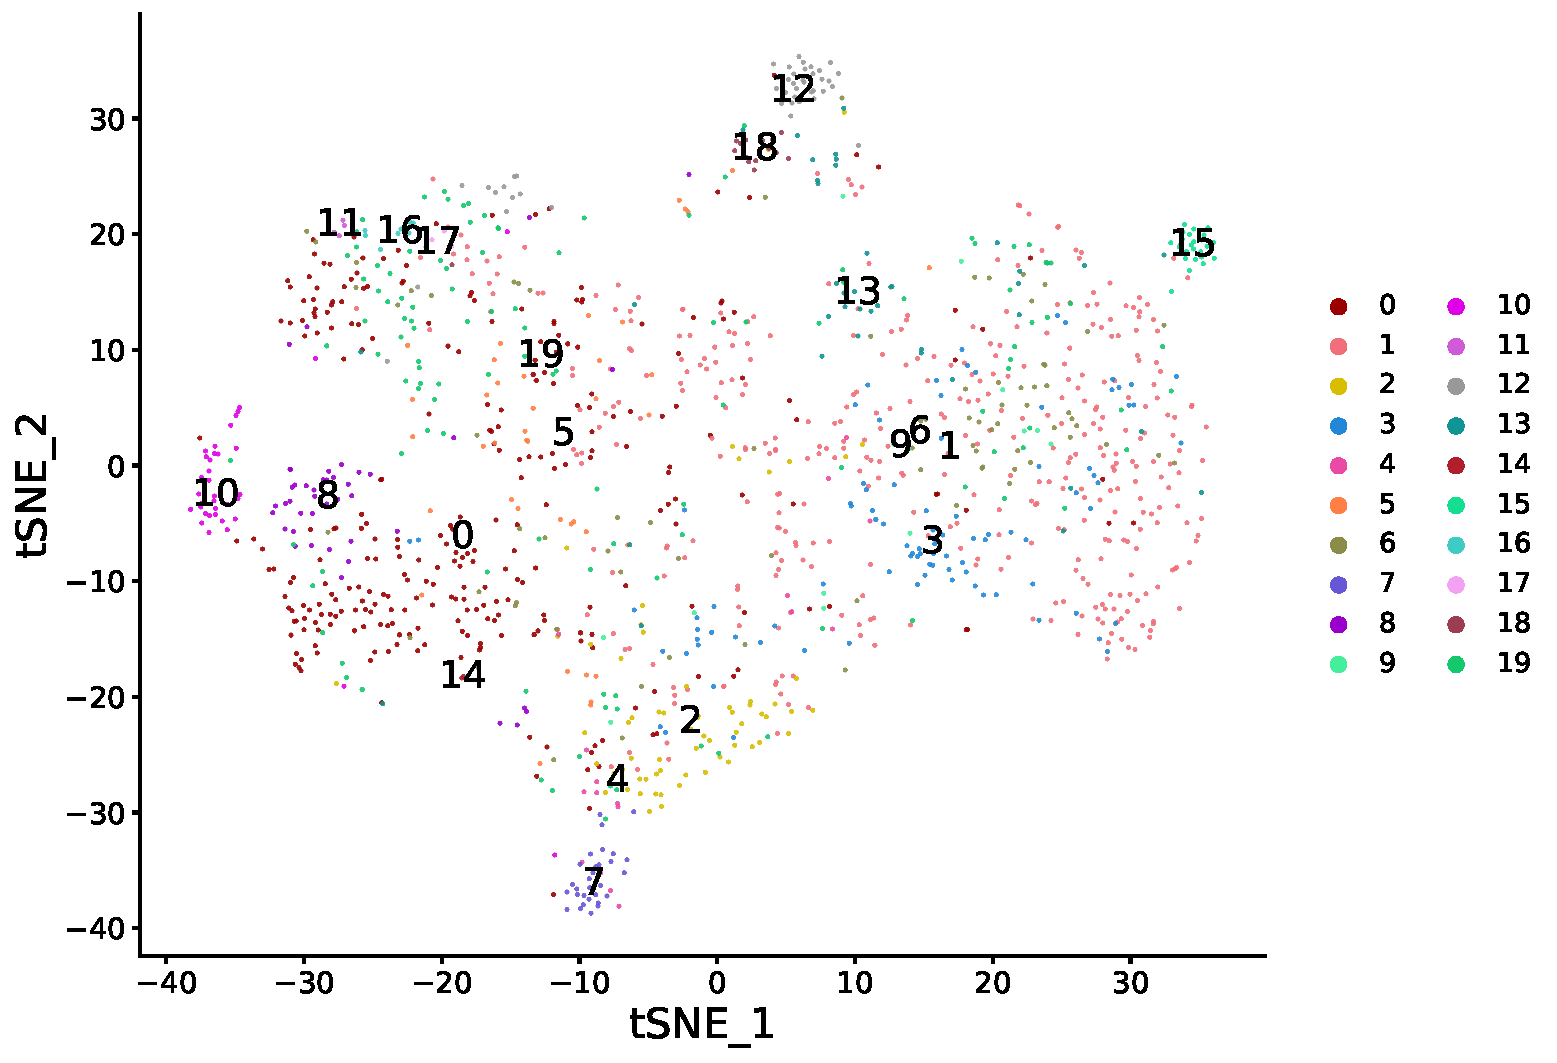
\includegraphics[width=0.45\textwidth]{fig_tsne_fedproto.pdf} &
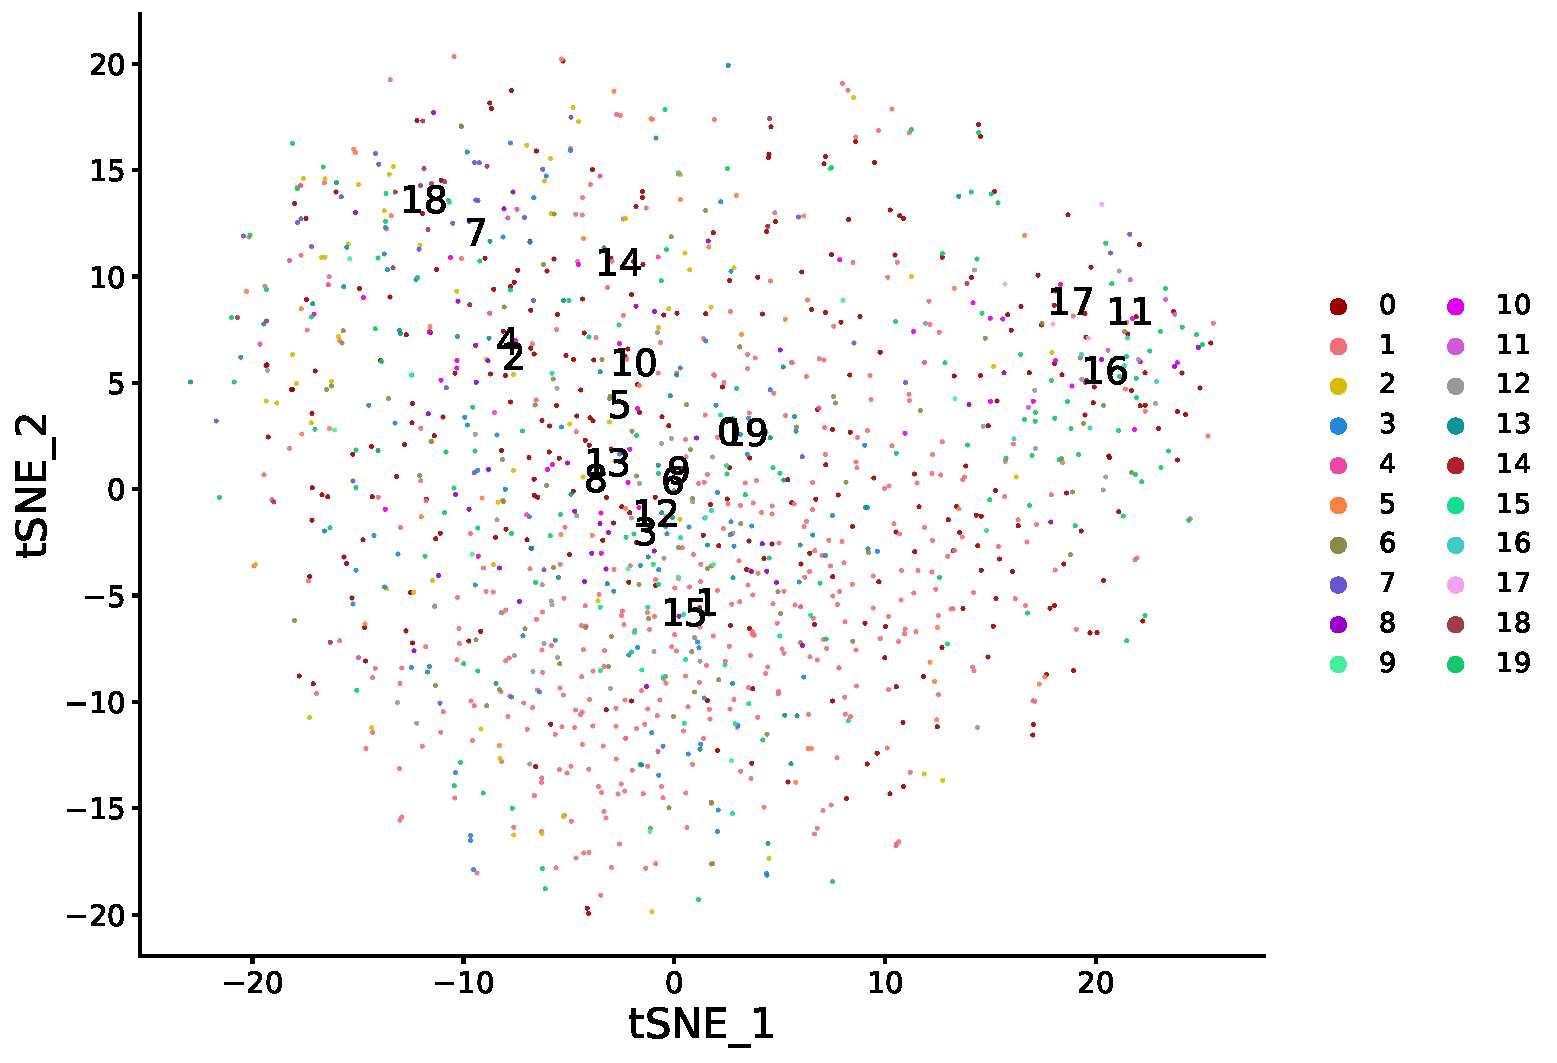
\includegraphics[width=0.45\textwidth]{fig_tsne_fedgmkd.pdf} \\[2pt]
{\small (a) FedProto} & {\small (b) FedGMKD} \\[8pt]
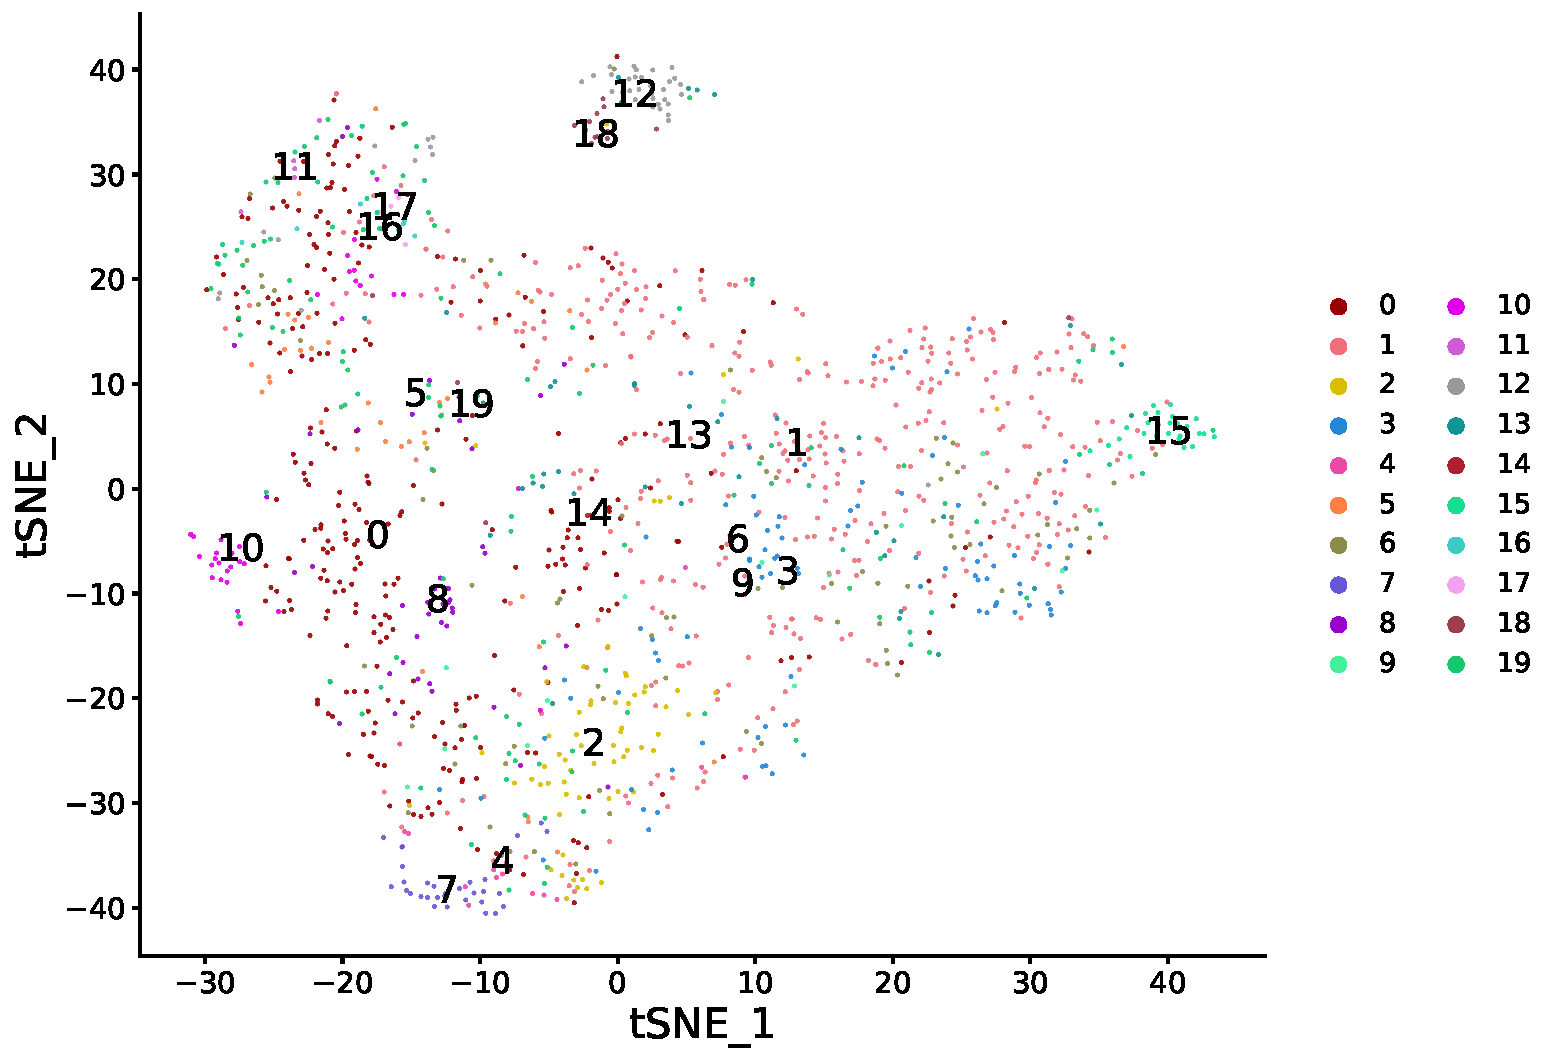
\includegraphics[width=0.45\textwidth]{fig_tsne_fedseproto.pdf} &
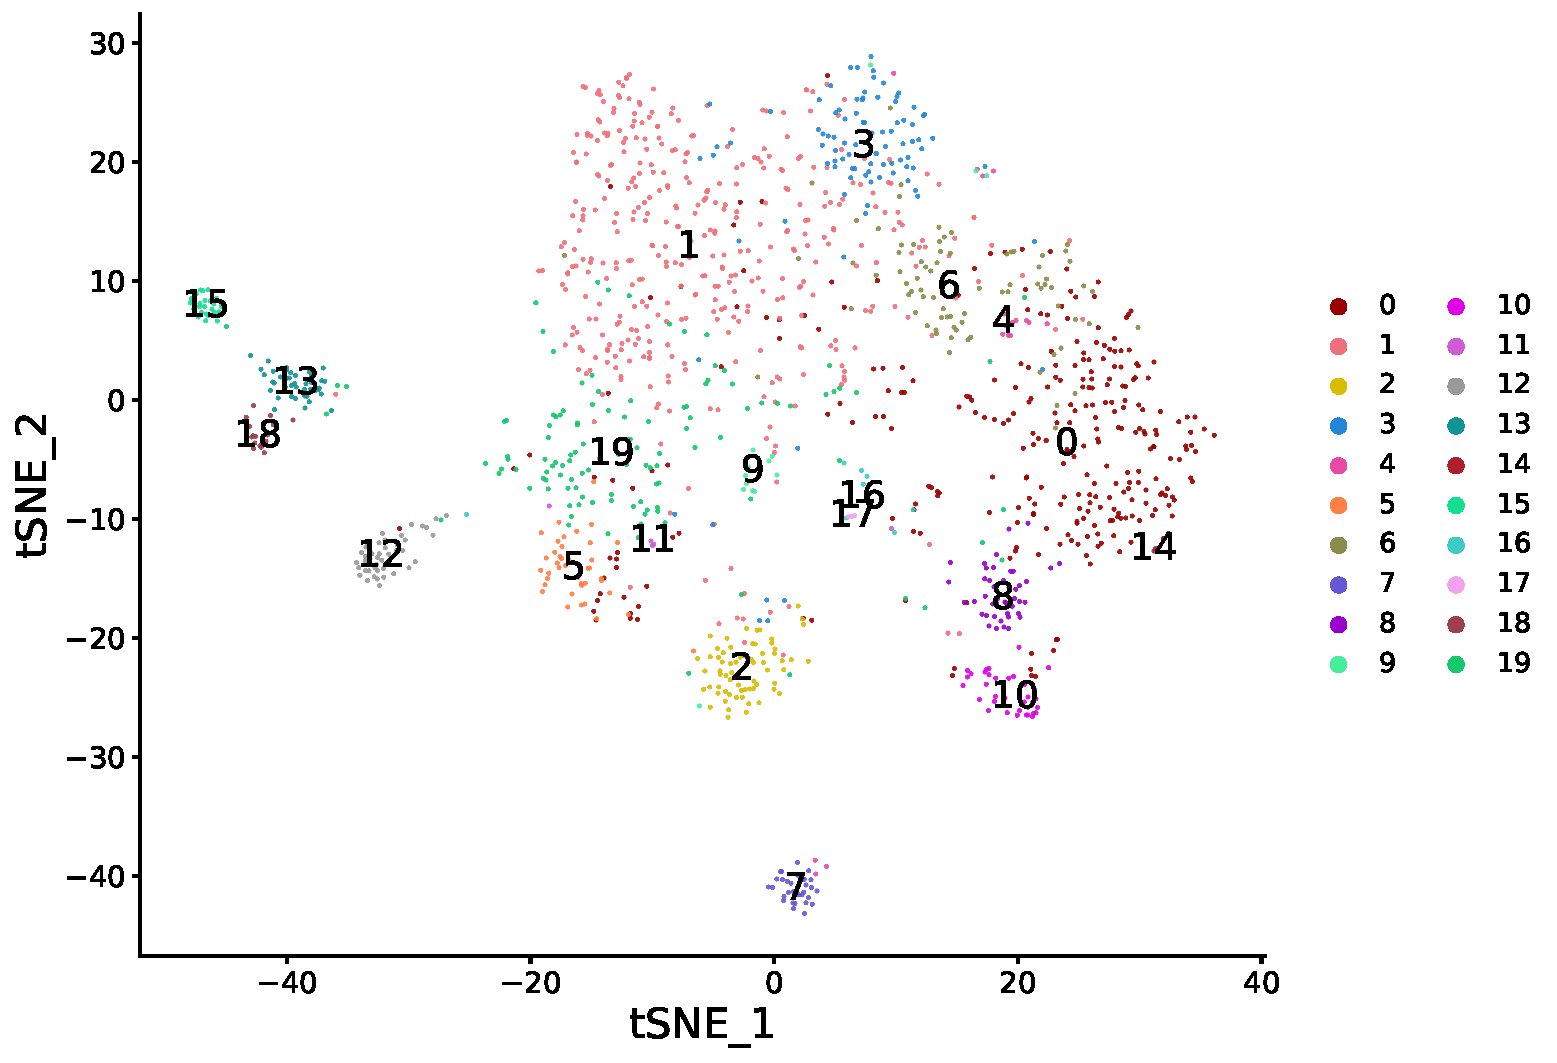
\includegraphics[width=0.45\textwidth]{fig_tsne_fedcop.pdf} \\[2pt]
{\small (c) FedSeProto} & {\small (d) FedCoP (ours)} \\
\end{tabular}
\caption{t-SNE of sample embeddings for four prototype-based federated methods on MuReD (single-label samples, 20 retinal pathology classes; marker color = class).}
\label{fig:tsne}
\end{figure}

Figure~\ref{fig:tsne} reveals a qualitative difference in how the four methods organize the embedding space. In the three baseline methods (FedProto, FedGMKD, FedSeProto), class clusters are scattered with no apparent structure governing their relative positions: classes that clinically co-occur (e.g., diabetic retinopathy and macular edema) are not systematically placed near each other, and the inter-class geometry is essentially an artifact of random initialization and independent per-class optimization. FedCoP, in contrast, exhibits a visibly more structured layout in which known co-occurring pathologies occupy adjacent regions of the embedding. This is the geometric signature of $L_{co}$: by aligning the prototype cosine Gram matrix to the federated co-occurrence correlation $\Rhat$, the loss actively pulls prototypes of co-occurring classes into nearby directions and pushes mutually exclusive ones apart. The result is an embedding space whose topology reflects clinical comorbidity rather than leaving it to chance.

Two additional observations are worth noting. First, the structure emerges despite the fact that no single client ever sees all 20 classes (each client receives only $\text{ways}=15$ under the non-IID partition), confirming that the co-occurrence signal is recovered through federated aggregation rather than from any local view---a direct empirical corroboration of Proposition~\ref{prop:estimation}(c). Second, FedGMKD's GMM prototypes and FedSeProto's semantic-domain decoupling both produce scattered layouts comparable to FedProto's, indicating that distributional representations and domain separation alone, without an explicit inter-class geometry target, do not impose structure on the embedding. This is consistent with the theoretical claim that conditional independence is the default: unless a mechanism actively encodes label dependence, the model has no reason to place co-occurring classes together.

% =====================================================================
\section{Conclusion}
\label{sec:conclusion}

We argued that pathology co-occurrence is an intrinsically federated quantity, invisible to any single client that sees only a subset of the $C$ classes and recoverable only by aggregation of label sufficient statistics, and we made it a first-class object of the federation. FedCoP estimates this structure federatedly and uses it on both sides of the pipeline: a structure loss aligns prototype geometry to the estimated correlation, and a mean-field decoder propagates evidence across co-occurring classes at inference. The theory says the independent decoder everyone uses is Bayes-optimal only under conditional independence and that the mean-field decoder is never worse and strictly better when the estimate tracks the residual correlation, while the federated estimator is unbiased under participation reweighting, concentrates, and is unrecoverable by any single client. The method is deliberately minimal, replacing two heuristic regularizers with one label-statistics-driven target, and the ablations separate the contributions of the federated structure, the training-side loss, the inference-side decoder, and six supplementary design choices.

Two limitations are worth stating. First, $\Rhat$ approximates the residual correlation $\Sigmay$ rather than equaling it; the shrinkage hedges this mismatch, but a feature-conditional estimator of $\Sigmay$ would tighten the theory. Second, the non-recoverability argument assumes each client's class support is a strict subset of all classes; when supports overlap substantially, local estimates become informative and the federated gain narrows, which is consistent with the smaller MuReD gains. Extending the estimator to the conditional regime and to streaming participation are natural next steps.

% =====================================================================
\begin{thebibliography}{99}
\setlength{\itemsep}{2pt}

\bibitem{an2024fedalc}
An, B., Li, B., Wei, M., Liu, S., Wang, Y., Tao, D., and Yan, Y.
\newblock Federated learning with only positive labels by exploring label correlations.
\newblock arXiv preprint arXiv:2404.15598, 2024.

\bibitem{caro2022mured}
Caro, M., Messina, P., Pino, P., Parra, D., and Mery, D.
\newblock MuReD: A multi-label retinal diseases dataset.
\newblock In \emph{Medical Image Computing and Computer Assisted Intervention (MICCAI)}, 2022.

\bibitem{chen2021fedbe}
Chen, H.-Y., Chao, W.-L., et al.
\newblock FedBE: Making Bayesian model ensemble applicable to federated learning.
\newblock In \emph{International Conference on Learning Representations (ICLR)}, 2021.

\bibitem{dembczynski2012labeldependence}
Dembczy\'nski, K., Waegeman, W., Cheng, W., and H\"ullermeier, E.
\newblock On label dependence and loss minimization in multi-label classification.
\newblock \emph{Machine Learning}, 88(1--2):5--45, 2012.

\bibitem{he2016resnet}
He, K., Zhang, X., Ren, S., and Sun, J.
\newblock Deep residual learning for image recognition.
\newblock In \emph{IEEE Conference on Computer Vision and Pattern Recognition (CVPR)}, 2016.

\bibitem{hinton2002poe}
Hinton, G.~E.
\newblock Training products of experts by minimizing contrastive divergence.
\newblock \emph{Neural Computation}, 14(8):1771--1800, 2002.

\bibitem{irvin2019chexpert}
Irvin, J., Rajpurkar, P., Ko, M., Yu, Y., et al.
\newblock CheXpert: Automated chest radiograph interpretation with deep learning.
\newblock In \emph{AAAI}, 2019.

\bibitem{jaeger2023chestxray}
Jaeger, S., Candemir, S., Antani, S., W\'ang, Y.-X.~J., Lu, P.-X., and Thoma, G.
\newblock Two public chest X-ray datasets for computer-aided screening of cardiopulmonary diseases.
\newblock \emph{Scientific Data}, 2023.

\bibitem{kairouz2021advances}
Kairouz, P., McMahan, H.~B., Avent, B., et al.
\newblock Advances and open problems in federated learning.
\newblock \emph{Foundations and Trends in Machine Learning}, 14(1--2):1--210, 2021.

\bibitem{li2020fedprox}
Li, T., Sahu, A.~K., Zaheer, M., Sanjabi, M., Talwalkar, A., and Smith, V.
\newblock Federated optimization in heterogeneous networks.
\newblock In \emph{MLSys}, 2020.

\bibitem{li2021fedbn}
Li, X., Jiang, M., Zhang, X., Kamp, M., and Dou, Q.
\newblock FedBN: Federated learning on non-IID features via local batch normalization.
\newblock In \emph{International Conference on Learning Representations (ICLR)}, 2021.

\bibitem{mcmahan2017fedavg}
McMahan, B., Moore, E., Ramage, D., Hampson, S., and Arcas, B.~A.
\newblock Communication-efficient learning of deep networks from decentralized data.
\newblock In \emph{AISTATS}, 2017.

\bibitem{rajpurkar2017chexnet}
Rajpurkar, P., Irvin, J., Zhu, K., Yang, B., et al.
\newblock CheXNet: Radiologist-level pneumonia detection on chest X-rays with deep learning.
\newblock arXiv:1711.05225, 2017.

\bibitem{read2011classifier}
Read, J., Pfahringer, B., Holmes, G., and Frank, E.
\newblock Classifier chains for multi-label classification.
\newblock \emph{Machine Learning}, 85(3):333--359, 2011.

\bibitem{sun2024fedmlp}
Sun, J., et al.
\newblock FedMLP: Federated multi-label medical image classification under task heterogeneity.
\newblock In \emph{Medical Image Computing and Computer Assisted Intervention (MICCAI)}, 2024.

\bibitem{tan2022fedproto}
Tan, Y., Long, G., Liu, L., Zhou, T., Lu, Q., Jiang, J., and Zhang, C.
\newblock FedProto: Federated prototype learning across heterogeneous clients.
\newblock In \emph{AAAI}, 2022.

\bibitem{tropp2015matrix}
Tropp, J.~A.
\newblock An introduction to matrix concentration inequalities.
\newblock \emph{Foundations and Trends in Machine Learning}, 8(1--2):1--230, 2015.

\bibitem{wainwright2008variational}
Wainwright, M.~J. and Jordan, M.~I.
\newblock Graphical models, exponential families, and variational inference.
\newblock \emph{Foundations and Trends in Machine Learning}, 1(1--2):1--305, 2008.

\bibitem{zhang2007mlknn}
Zhang, M.-L. and Zhou, Z.-H.
\newblock ML-$k$NN: A lazy learning approach to multi-label classification.
\newblock \emph{ACM Transactions on Knowledge Discovery from Data}, 1(2):7, 2007.

\bibitem{wang2017chestxray8}
Wang, X., Peng, Y., Lu, L., Lu, Z., Bagheri, M., and Summers, R.~M.
\newblock ChestX-ray8: Hospital-scale chest X-ray database and benchmarks on weakly-supervised classification of common thorax diseases.
\newblock In \emph{IEEE Conference on Computer Vision and Pattern Recognition (CVPR)}, 2017.

\bibitem{zhang2024fedgmkd}
Zhang, J., Shan, J., and Han, B.
\newblock FedGMKD: An efficient prototype federated learning framework through knowledge distillation and discrepancy-aware aggregation.
\newblock In \emph{Advances in Neural Information Processing Systems (NeurIPS)}, 2024.

\bibitem{fedseproto2024}
FedSeProto: Federated learning with semantic-aware prototypes over heterogeneous clients.
\newblock In \emph{European Conference on Artificial Intelligence (ECAI)}, 2024.

\end{thebibliography}

\end{document}
